\section{Arquitectura}

En esta sección presentamos y analizamos la arquitectura diseñada para resolver las funcionalidades requeridas, conciliando a la vez las necesidades presentadas por los atributos de calidad y el análisis de riesgos.

\subsection{Comunicación con Drones}

Para el monitoreo de los cultivos se utilizan drones que toman fotografías de los terrenos, las cuales se procesan para extraer las mediciones necesarias sobre el estado de salud de las plantas.  Para esto, se cuenta con un componente dedicado a la comunicación con las interfaces de manejo de drones que nos proveen tanto el Ministerio como la empresa privada. Por defecto se prioriza la utilización del sistema de drones estatales, mientras que en caso de no responder a los pedidos se utiliza la red privada. Para atacar el problema de que los drones no tengan conectividad - y no se puedan recibir las imágenes tomadas por los mismos - se proveen repositorios temporales de imágenes en los nodos distribuidos de ArSat para que los aparatos descarguen las fotos tomadas. Luego, esta información se replica y reorganiza de acuerdo a la ubicación del acceso más frecuente.\\
\indent El componente encargado del pedido de imágenes busca en el repositorio de pedidos y, gracias al repositorio de geolocalización, envía la latitud y longitud que se desea analizar. A medida que se reciben las imágenes, se pasan al geolocalizador utilizando una cola que se encarga de identificar el tipo de cultivo analizando las imágenes y usando la información del repositorio de geolocalizaciones. Este componente se encarga también de descartar las imágenes erróneas que no permitan un posterior análisis correcto. El repositorio contiene información ingresada por los usuarios sobre la localización de las plantaciones, así como su estado. Esta información se utiliza para comparar con el análisis que haga el geolocalizador y poder verificar de qué plantación se trata. Una vez taggeada, la imagen se envía a los analizadores que trabajan en paralelo para reconocer la temperatura, el estado del suelo y la salinidad del agua. Eventualmente podrían agregarse más filtros para que analicen otras bandas espectrales de las fotos. Vale observar que este conjunto de componentes (los analizadores y el geolocalizador) tienen varias instancias corriendo en simultáneo para mejorar la performance. Luego de esto se procede a unificar los resultados, comprimir las imágenes tomadas y guardar en el repo de información de manera encriptada.\\

\begin{figure}[h!]
  \centering
  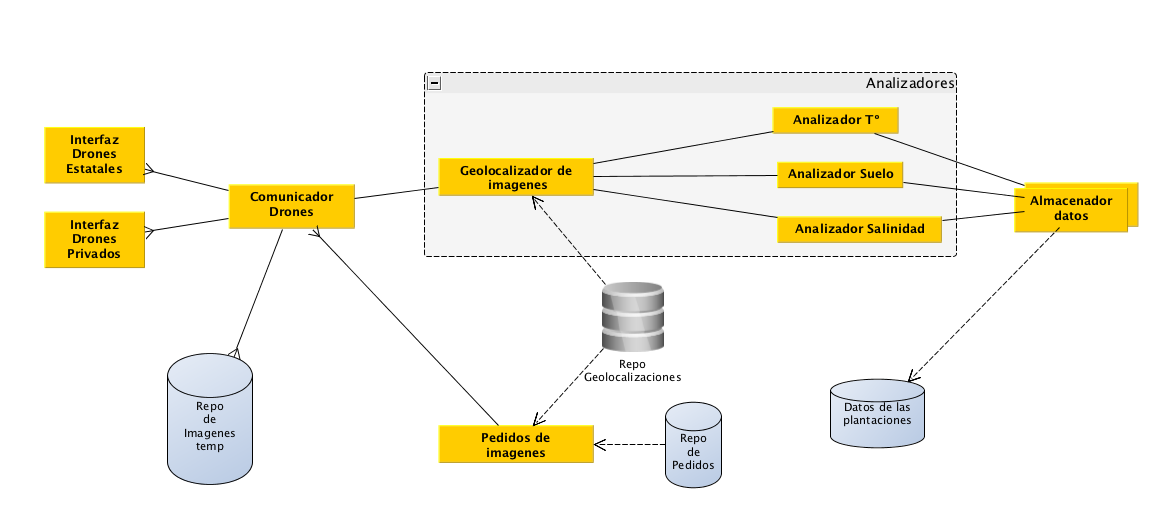
\includegraphics[width=1\textwidth]{./images/arq_drones.png}
  \caption{Arquitectura de comunicación con drones y procesamiento de imágenes}
  \label{fig:clases4}
\end{figure}

\subsection{Comunicación con estaciones meteorológicas}

El mecanismo es bastante similar a la comunicación con drones. Existe un repositorio de pedidos de clima que puede haber sido poblado por el usuario o por el sistema de monitoreo automático. El comunicador de estación meteorológica establece el pedido a la interfaz meteorológica definida y luego envía el paquete usando una cola al analizador, quien luego se lo envía al almacenados de datos que lo agrega al repo. Como primera opción se accede a los servidores meteorológicos del INTA, pero en caso de fallas se utiliza una cadena de opciones alternativas para obtener otros datos, aunque no sean tan precisos. Además, como última opción ante las fallas se envía un mail informando de este problema.

\begin{figure}[h!]
  \centering
  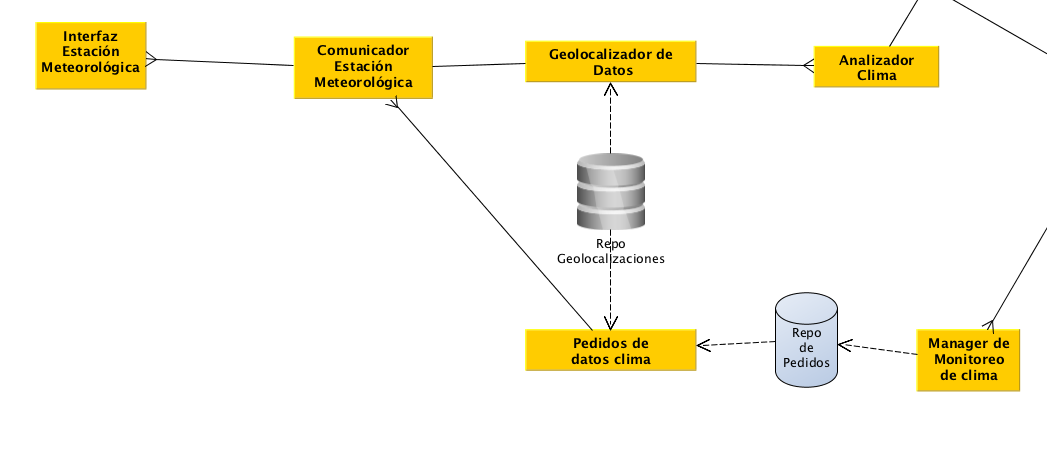
\includegraphics[width=1\textwidth]{./images/arq_clima.png}
  \caption{Arquitectura de comunicación con estaciones meteorológicas y procesamiento de datos}
  \label{fig:clases4}
\end{figure}


\subsection{Comunicación con Interfaz de usuarios}

La interfaz de usuario cuenta con autenticación para asegurar el acceso a la aplicación y un sistema de logging de entradas al sistema para registrar los accesos.
Utilizando la interfaz de usuario, se permite agregar datos sobre las plantaciones de manera manual. También se realiza la configuración de monitoreo de clima y de imágenes (frecuencia, horarios, etc). A su vez, se guarda un log de los cambios en la configuración que se hagan. El visualizados de datos utiliza la información del repo de datos de plantaciones para mostrar en pantalla el estado actual de las plantaciones.
Por último, el manager de monitoreo de imágenes  y de clima, se encarga de ir agregando los pedidos que deben realizarse para que luego se vayan realizando. Para esto está el repo de pedidos dónde el componente que pide las imágenes se conecta de manera blackboard y luego realiza la solicitud usando el comunicador con los drones.

\begin{figure}[h!]
  \centering
  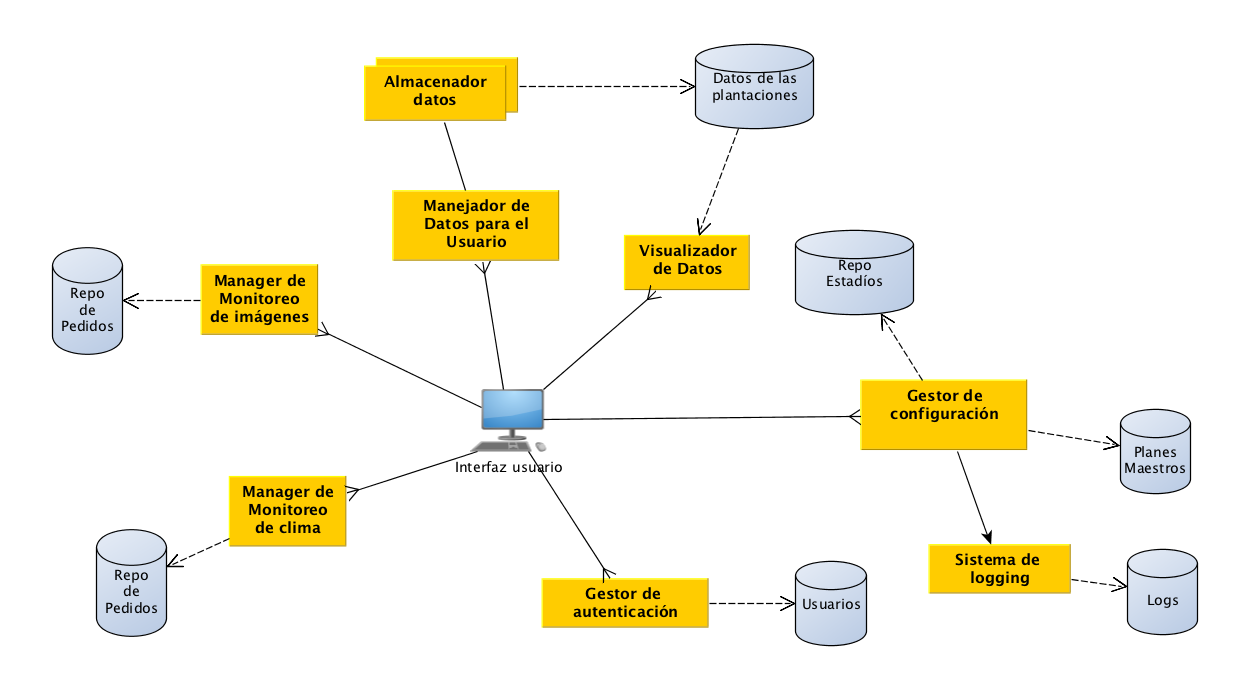
\includegraphics[width=0.8\textwidth]{./images/arq_interfazusuario.png}
  \caption{Arquitectura de comunicación con la interfaz de usuario}
  \label{fig:clases4}
\end{figure}

\subsection{Planificación}

Con la información almacenada en los repositorios, el planificador arma los eventos que deben realizarse para continuar con el plan de trabajo deseado. Luego el manager de actuadores se encarga de enviar el pedido a los distintos actuadores. Todos los eventos se guardan en un repositorio para permitir la auditabilidad en caso de que sea necesario. El controlador de estadiós se encarga de ir cambiando el estado de las plantas en base a los datos que se obtienen y al plan maestro.

\begin{figure}[h!]
  \centering
  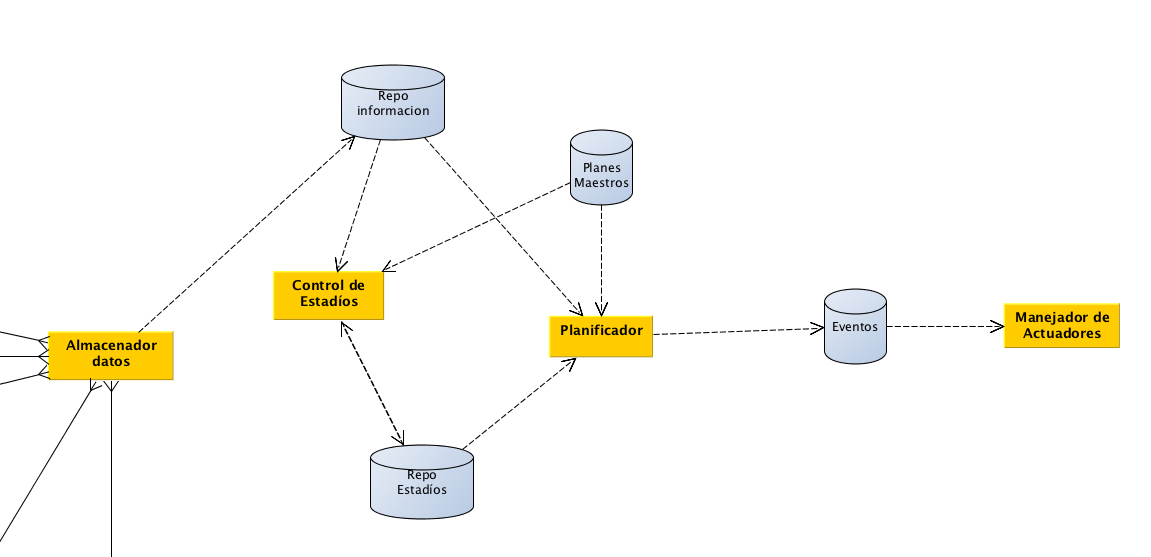
\includegraphics[width=1\textwidth]{./images/arq_plan.png}
  \caption{Arquitectura de planificación de eventos}
  \label{fig:clases4}
\end{figure}
